\chapter{에너지와 해밀토니안}

\lectureoverview{먼저 능동 대칭의 의미를 더 정확히 규정하고, 병진과 회전이 운동량과 각운동량을 어떻게 생성하는지 살펴본다. 빠져 있던 보존량은 에너지다. 에너지에 대응하는 대칭은 시간 병진이며, 그 보존량은 해밀토니안 \(H=\sum_i p_i\dot q_i-L\)이다. 이 유도 과정은 명시적인 시간 의존성이 선택한 부분계와 그 환경 사이에서 에너지를 어떻게 전달하는지도 정확히 보여 준다.}

\section{정식 논증에 앞서 나온 질문}

이후 주제를 다루는 데 필요한 고전역학의 최소한에 가까워지고 있지만, 더 배울 가치가 있는 역학은 아직 많이 남아 있다. 본격적인 논증에 앞서 두 가지 질문이 나왔다.

\begin{classroomqa}
  \audiencequestion{이 입문 강의 다음에는 어떤 책이 도움이 되나요?
  \lecturetimestamp{00:00:36--00:02:13}}
  \lecturerresponse{널리 쓰이는 고급 참고서는 Herbert Goldstein의 \emph{고전역학}이다. 역학의 변분 원리를 다룬 Cornelius Lanczos의 책도 관련 참고 자료다. 한 강사가 이용 가능한 모든 교재를 훑어볼 수 있다고 가장하기보다는 강의용 독서 목록을 참고하는 편이 더 유용하다.}
\end{classroomqa}

두 번째 질문에는 아직 해결되지 않은 측정 문제의 당시 상황이 담겨 있다. 2011년에 OPERA 실험은 CERN에서 Gran Sasso로 보낸 중성미자가 예상보다 일찍 도착한 듯한 결과를 보고했다. 보고된 시간 차이는 중성미자를 만들 때 사용한 양성자 펄스보다 짧았다. 따라서 시간 분석에서는 중성미자가 방출될 때 하나를 표시해 두었다가 검출 시 같은 입자인지 확인하는 대신 펄스의 시간 분포를 비교해야 했다.

\begin{classroomqa}
  \audiencequestion{빛보다 빠른 중성미자라는 결과는 해결되었나요?
  \lecturetimestamp{00:02:30--00:09:03}}
  \lecturerresponse{당시에는 어떤 결론도 내릴 근거가 없었다. 빔 펄스의 형태, 표적의 가열, 동기화 문제를 모두 기술적으로 면밀히 검토해야 했다. 한 가지 추측성 제안에서는 GPS 위성의 운동을 고려했다. 위성 좌표계에서는 시간 신호가 전달되는 동안 발생원과 검출기가 움직이므로 수십 나노초 정도의 보정이 생긴다는 것이었다. 이 추산은 차수 크기를 따져 보는 연습으로는 흥미로웠지만, 실험 결과를 그럴듯하게 진단한 것으로 제시되지는 않았다. 해당 속도에서의 통상적인 로런츠 수축은 보고된 효과를 설명하기에 너무 작았다. 적절한 대응은 실험 분석을 기다리는 것이었다.}
\end{classroomqa}

\begin{figure}[htbp]
  \centering
  \includegraphics[width=0.78\textwidth]{lecture_05_figure_07.png}
  \caption{역사적 중성미자 측정 문제를 논의하며 살펴본 위성 좌표계의 시간 측정 도식.}
  \lectureframe{00:06:30}
\end{figure}

시간 측정에 관한 논의는 아래 역학 내용을 이해하는 데 필요하지 않다. 하지만 그럴듯한 규모 추산과 확립된 실험적 설명은 서로 다르다는 점을 상기시켜 준다.

\section{능동 대칭과 계의 선택}

앞선 논의에서 충분히 명확히 다루지 못한 문제로 돌아가 보자. 대칭이란 정확히 무엇인가? 직선 위의 입자와 다음 지시를 생각하자.
\begin{equation}
  x\longrightarrow x+1.
  \label{eq:l5-shift-one}
\end{equation}
이를 이해하는 방법은 두 가지다. \emph{수동} 변환은 직선 위의 점에 붙인 이름을 다시 정하는 것이다. 한때 \(x=0\)이라고 부르던 점을 이제 \(x'=1\)이라고 부를 수 있지만, 입자가 움직인 것은 아니다. \emph{능동} 변환은 표지를 그대로 둔 채 입자 자체를 \(x\)에서 \(x+1\)로 이동시킨다. 외부 퍼텐셜에 대한 입자의 위치를 바꾸는 것은 두 번째 작용뿐이다.

\begin{figure}[htbp]
  \centering
  \includegraphics[width=0.82\textwidth]{lecture_05_figure_08.png}
  \caption{규칙 \(x\mapsto x+1\), 고정된 좌표축, 외부 퍼텐셜을 이용하면 능동적 운동과 수동적 표지 재설정을 구별할 수 있다.}
  \lectureframe{00:11:20}
\end{figure}

\begin{classroomqa}
  \audiencequestion{입자를 움직여 퍼텐셜 에너지가 달라진다면, 그 퍼텐셜의 발생원은 계에서 제외한 건가요?
  \lecturetimestamp{00:12:19--00:14:18}}
  \lecturerresponse{그렇다. 계를 ``퍼텐셜 안의 입자''라고 부르면, 세계를 입자와 퍼텐셜 \(V(x)\)를 만들어 내는 지구 같은 무거운 환경으로 나누는 것이다. 지구도 반동하지만, 이 근사에서는 질량이 엄청나게 커서 그 반동을 무시할 수 있다. 고정된 지구에 대해 입자를 움직이면 \(V\)가 달라질 수 있지만, 입자와 지구를 함께 병진시키면 달라지지 않는다.}
\end{classroomqa}

\begin{classroomqa}
  \audiencequestion{앞서 회전을 예로 들었을 때 위치뿐 아니라 속도도 바뀌었나요?
  \lecturetimestamp{00:14:26--00:15:29}}
  \lecturerresponse{그렇다. 강체의 능동 회전은 한 순간의 위치에만 작용하는 것이 아니라 전체 이력에 작용한다. 위치 벡터와 속도 벡터가 모두 회전한다. 반면 모든 시각에 똑같이 적용하는 상수 병진은 \(x\)를 바꾸지만 \(\dot x\)는 바꾸지 않는다.}
\end{classroomqa}

계와 환경의 구분은 두 번 더 등장한다. 시간에 따라 변하는 장치가 부분계와 에너지를 주고받을 때, 그리고 거시적 마찰 때문에 관측되지 않는 미시적 운동에 에너지가 숨을 때다.

\section{배치 공간에서의 무한소 운동}

일반적인 역학계의 배치는 일반화 좌표 \(q_i\) 공간의 한 점이다. 능동적인 무한소 변환은 가능한 모든 배치를 그에 가까운 배치로 옮긴다. 이를 다음과 같이 쓴다.
\begin{equation}
  \delta q_i=\epsilon f_i(q),
  \label{eq:l5-general-transformation}
\end{equation}
함수 \(f_i\)는 배치 공간에서 하나의 고정된 변위장을 지정한다. 이 함수들은 모든 좌표에 의존할 수 있으며, 일부는 사라질 수 있다. 공통 인자 \(\epsilon\)는 작으며, 변환 단계의 크기와 변환의 형태를 분리한다.

\begin{figure}[htbp]
  \centering
  \includegraphics[width=0.75\textwidth]{lecture_05_figure_09.png}
  \caption{배치 공간의 각 점에 붙인 변위 벡터.}
  \lectureframe{00:16:50}
\end{figure}

\begin{figure}[htbp]
  \centering
  \includegraphics[width=0.80\textwidth]{lecture_05_figure_10.png}
  \caption{좌표에 따라 달라지는 무한소 변환 \(\delta q_i=\epsilon f_i(q)\).}
  \lectureframe{00:18:00}
\end{figure}

변환 규칙 자체에는 명시적인 시간 의존성이 없다. 따라서 속도에 작용하는 변환은 다음과 같다.
\begin{equation}
  \delta\dot q_i=\frac{d}{dt}(\delta q_i)
  =\epsilon\sum_j\frac{\partial f_i}{\partial q_j}\dot q_j.
  \label{eq:l5-velocity-variation}
\end{equation}
병진에서는 \(f_x=1\)이므로 \(\delta\dot x=0\)이다. 회전에서는 \(f_i\)가 위치에 따라 달라지므로 속도도 변한다.

\begin{classroomqa}
  \audiencequestion{마지막의 작은 인자 \(\delta q_i=\epsilon f_i(q)\)는 모든 점에서 같은 상수인가요?
  \lecturetimestamp{00:19:58--00:20:51}}
  \lecturerresponse{그렇다. 하나의 상수 \(\epsilon\)는 모든 좌표 변화가 동일한 작은 양의 1차가 되도록 하는 표기상의 장치다. 공간 의존성은 \(f_i(q)\)에 들어 있으며, \(\epsilon\)에는 들어 있지 않다. 이 함수들 자체는 작을 필요가 없다.}
\end{classroomqa}

\section{변환이 대칭이 되는 조건}

능동 변환은 일반적으로 퍼텐셜 에너지를 바꾼다. 운동에너지도 바뀔 수 있다. 곡선좌표에서 운동에너지 항은 다음 형태를 갖는다.
\begin{equation}
  T=\frac12\sum_{i,j}g_{ij}(q)\dot q_i\dot q_j,
  \label{eq:l5-kinetic-metric}
\end{equation}
따라서 배치 공간에서 움직이면 그 계수가 달라질 수 있다. 극좌표에서 익숙한 \(r^2\dot\theta^2\) 항이 가장 간단한 예다.

여기서 변환이 대칭이라는 것은 \emph{전체} 라그랑지안의 변화가 1차에서 사라진다는 뜻이다.
\begin{equation}
  \delta L=O(\epsilon^2),
  \label{eq:l5-symmetry-condition}
\end{equation}
이 조건은 특정한 해 하나가 점유하는 배치에서만이 아니라 배치 공간의 모든 점에서 성립해야 한다.

예를 들어, \(x\mapsto x+\epsilon\) 변환에서는
\begin{equation}
  \delta V=\frac{\partial V}{\partial x}\epsilon.
  \label{eq:l5-potential-variation}
\end{equation}
이 값이 가능한 모든 \(x\)에 대해 사라진다면,
\(\partial V/\partial x=0\)이다. 즉, 퍼텐셜은 \(x\)에 의존하지 않는다. 모든 공간 방향의 병진 변환에도 퍼텐셜이 변하지 않는다면, 퍼텐셜은 상수이다.

\begin{figure}[htbp]
  \centering
  \includegraphics[width=0.80\textwidth]{lecture_05_figure_11.png}
  \caption{\(x\) 병진을 \(x\)에 의존하지 않는 퍼텐셜 \(V(y)\)에 적용한 경우.}
  \lectureframe{00:23:40}
\end{figure}

매끄러운 1매개변수 군에서는 모든 점에서 1차 변화가 사라지므로, 무한소 단계를 이어 붙여 유한 대칭을 만들 수 있다.

\begin{classroomqa}
  \audiencequestion{운동에너지와 퍼텐셜 에너지가 각각 따로 불변이어야 하나요?
  \lecturetimestamp{00:24:44--00:25:33}}
  \lecturerresponse{아니다. 불변이어야 하는 것은 전체 라그랑지안뿐이다. 일부 라그랑지안에는 좌표와 속도가 섞인 항이 들어 있어 --, \(T\), \(V\)로 유용하게 분리할 수 없다. 그러므로 각 항의 불변성을 따지는 질문 자체가 의미 없을 수도 있다.}
\end{classroomqa}

\begin{classroomqa}
  \audiencequestion{``변화가 없다''는 말은 정확히 변화가 없다는 뜻인가요, 아니면 무시할 만큼 작다는 뜻인가요?
  \lecturetimestamp{00:25:34--00:28:59}}
  \lecturerresponse{무한소 변환에서는 \(\epsilon\)에 비례하는 항이 없다는 뜻이다. 국소 계산에서는 \(\epsilon^2\) 차수의 항을 버린다. 1차 조건이 1매개변수 궤도를 따라 모든 점에서 성립하므로 국소 단계를 반복하면 유한 불변성이 얻어진다.}
\end{classroomqa}

\section{운동량과 각운동량의 재도출}

여기서 다루는 정확한 시간 독립 점 대칭에 대해 앞서 증명한 결과는 다음과 같다.
\begin{equation}
  Q=\sum_i p_i f_i(q),
  \qquad
  p_i=\frac{\partial L}{\partial\dot q_i},
  \qquad
  \dot Q=0.
  \label{eq:l5-noether-charge}
\end{equation}
인자 \(\epsilon\)는 \(Q\)에 포함되지 않는다. 대칭 궤도를 따라 얼마나 이동하는지를 나타낼 뿐이다.

\begin{figure}[htbp]
  \centering
  \includegraphics[width=0.82\textwidth]{lecture_05_figure_12.png}
  \caption{일반적인 무한소 변위와 이에 대응하는 보존 노에터 전하.}
  \lectureframe{00:30:00}
\end{figure}

\(x\) 방향 병진에서는 \(f_x=1\)이고 \(Q=p_x\)이다. 모든 병진 대칭이 성립하면 운동량의 세 성분이 모두 보존된다. 서로 상호작용하는 입자가 여러 개일 때는 모든 입자를 함께 병진시키는 것이 대칭이다. 상호작용이 상대 위치에만 의존하면 \begin{equation}
  \mathbf P=\sum_a\mathbf p_a
  \label{eq:l5-total-momentum}
\end{equation}가 보존된다. 입자 하나만 나머지 입자에 대해 움직이는 것은 대칭이 아니다.

\begin{figure}[htbp]
  \centering
  \includegraphics[width=0.80\textwidth]{lecture_05_figure_13.png}
  \caption{함께 병진시키면 운동량의 각 성분이 보존되어 총운동량이 보존된다.}
  \lectureframe{00:32:50}
\end{figure}

\(x\)-\(y\) 평면에서 무한소 회전을 생각하고, 회전 방향을 다음과 같이 정한다.
\begin{equation}
  \delta x=-y\epsilon,
  \qquad
  \delta y=x\epsilon.
  \label{eq:l5-planar-rotation}
\end{equation}
다음 식에서 알 수 있듯이 반지름은 보존된다.
\begin{equation}
  \delta(x^2+y^2)
  =2x\delta x+2y\delta y=0.
  \label{eq:l5-radius-invariance}
\end{equation}

\begin{figure}[htbp]
  \centering
  \includegraphics[width=0.76\textwidth]{lecture_05_figure_14.png}
  \caption{평면 무한소 회전의 기하학적 의미와 좌표 표현.}
  \lectureframe{00:35:05}
\end{figure}

식~\eqref{eq:l5-planar-rotation}을 미분하면 속도도 함께 회전한다. 따라서 \(\dot x^2+\dot y^2\)는 불변이고, 중심 퍼텐셜 \(V(\sqrt{x^2+y^2})\)은 라그랑지안 전체를 변하지 않게 한다. 이에 대응하는 전하는 다음과 같다.
\begin{equation}
  Q=-yp_x+xp_y=(\mathbf r\times\mathbf p)_z.
  \label{eq:l5-angular-charge}
\end{equation}

\begin{figure}[htbp]
  \centering
  \includegraphics[width=0.76\textwidth]{lecture_05_figure_15.png}
  \caption{회전에 대응하는 노에터 전하, 즉 각운동량의 \(z\) 성분.}
  \lectureframe{00:38:50}
\end{figure}

다른 좌표 평면에서의 회전은 나머지 성분을 준다. 여러 입자에 대해 보존되는 벡터는 다음과 같다.
\begin{equation}
  \mathbf J=\sum_a\mathbf r_a\times\mathbf p_a.
  \label{eq:l5-total-angular-momentum}
\end{equation}
중심 별의 퍼텐셜 안에서 움직이는 행성이 기본적인 예다. 모든 회전에 대한 불변성은 각운동량의 모든 성분이 보존됨을 뜻한다.

\begin{classroomqa}
  \audiencequestion{한쪽에서의 미분값과 다른 쪽에서의 미분값이 다른 뾰족한 첨점에서는 어떻게 되나요?
  \lecturetimestamp{00:42:25--00:44:21}}
  \lecturerresponse{타당한 지적입니다. 현재 논증은 미분 가능하고 도함수가 유일하게 정해지는 함수를 가정합니다. 매끄러운 극댓값 위에 놓인 물체처럼 불안정한 평형은 그 자체로 문제가 되지 않습니다. 그 점에서 도함수가 존재하고 사라지기 때문입니다. 실제 첨점을 다루려면 논증을 수정해야 합니다.}
\end{classroomqa}

\begin{classroomqa}
  \audiencequestion{변환 매개변수가 시간에 무관한데 회전하면 왜 속도가 바뀌나요?
  \lecturetimestamp{00:44:23--00:45:23}}
  \lecturerresponse{매개변수는 상수지만 변위장은 좌표에 의존한다. 일반적인 규칙은 \(\delta\dot q_i=d(\delta q_i)/dt\)이다. 병진에서는 \(\delta x\)가 상수지만 회전에서는 \(\delta x=-y\epsilon\)이므로 \(\delta\dot x=-\dot y\epsilon\)이다.}
\end{classroomqa}

\section{초등적인 운동에너지 빼기 퍼텐셜 에너지 형식을 넘어}

자기장이 없는 비상대론적 입자를 직교좌표로 나타내면 \(L=T-V\)이다. 더 일반적인 좌표에서는 식~\eqref{eq:l5-kinetic-metric}의 이차형식이 나온다. 자기장이 있으면 속도에 선형인 항, 개략적으로 \(\mathbf A(q)\cdot\dot{\mathbf q}\)가 들어가 좌표와 속도가 서로 섞인다. 이런 경우에는 모든 항을 통상적인 운동에너지와 퍼텐셜 에너지로 억지로 나누기보다 \(L(q,\dot q,t)\)를 하나의 함수로 다루는 편이 낫다.

\begin{figure}[htbp]
  \centering
  \includegraphics[width=0.80\textwidth]{lecture_05_figure_16.png}
  \caption{좌표에만 의존하는 퍼텐셜과 일반적인 좌표 의존 이차 운동에너지 항.}
  \lectureframe{00:47:20}
\end{figure}

\begin{classroomqa}
  \audiencequestion{라그랑지안이 운동에너지와 퍼텐셜 에너지로 깔끔히 분리되지 않을 수 있는 이유는 무엇인가요? 그래도 라그랑지안은 \(T-V\)로 정의되나요?
  \lecturetimestamp{00:45:26--00:48:13}}
  \lecturerresponse{장애물은 곡선좌표에서 비롯될 수도 있고, 자기력처럼 실제 속도 의존 상호작용에서 생길 수도 있다. 라그랑지안이 속도에 대한 이차형식에서 좌표에만 의존하는 함수를 뺀 형태일 때에만 두 항을 \(T\)와 \(V\)라고 부른다. 그렇지 않아도 라그랑지안은 여전히 \(q\)와 \(\dot q\)의 함수로서 완전히 타당하지만, 그렇게 나누는 것은 별로 유용하지 않다. 에너지의 올바른 일반적 정의는 해밀토니안에서 나온다.}
\end{classroomqa}

\begin{classroomqa}
  \audiencequestion{첫 모임에서 다룬 늘어진 사슬 예제는 최소작용 원리를 적용한 것이었나요?
  \lecturetimestamp{00:48:15--00:49:45}}
  \lecturerresponse{그 예제는 최소에너지로 정해지는 평형 문제였지, 정지작용으로 선택되는 이력 문제는 아니었다. 통상적인 \(T-V\) 계의 정적 해에서는 \(\dot p_i=0\)이므로 오일러--라그랑주 방정식은 퍼텐셜의 정지점 조건인 \(\partial V/\partial q_i=0\)로 줄어든다.}
\end{classroomqa}

운동량과 각운동량은 이제 공간 대칭과 연결되었다. 뚜렷하게 빠져 있는 양은 에너지다.

\section{시간 병진 불변성}

\(t_0\)에 시작해 \(t_1\)에 끝나며 어떤 결과를 내는 실험을 생각하자. 같은 준비를 한 뒤, 더 늦은 시점인 \(t_0+\Delta t\)에 시작해 \(t_1+\Delta t\)에 끝나도록 반복한다. 결과가 변하지 않는다면 그 계는 시간에 대한 능동 병진에 불변이다.

\begin{figure}[htbp]
  \centering
  \includegraphics[width=0.82\textwidth]{lecture_05_figure_17.png}
  \caption{배치 공간의 이력 안에서 실험과 이를 시간 병진시킨 실험을 나타낸 그림.}
  \lectureframe{00:52:45}
\end{figure}

축전기 판 사이의 하전 입자는 이 대칭이 깨지는 예다. 판의 전하가 고정되어 있다면 같은 실험을 언제든 수행할 수 있다. 외부 발전기가 판을 계속 충전한다면, 입자가 방출되는 시점에 따라 입자가 경험하는 전기장이 달라진다. 이때 입자는 명시적으로 구동되는 부분계다.

\begin{figure}[htbp]
  \centering
  \includegraphics[width=0.82\textwidth]{lecture_05_figure_18.png}
  \caption{시간 병진 도식 옆에 대비해 그린, 전하가 고정된 축전기 판과 외부 작용으로 변하는 축전기 판.}
  \lectureframe{00:54:45}
\end{figure}

진동자에서도 같은 점을 볼 수 있다.
\begin{equation}
  L=\frac12m\dot x^2-\frac12k(t)x^2.
  \label{eq:l5-driven-oscillator}
\end{equation}
외부 전기장이나 자기장이 물질을 서서히 변화시켜 유효 용수철 상수를 바꿀 수 있다. \(k\)가 변하면 진동자 실험을 시간상으로 옮겼을 때 결과가 달라진다.

\begin{figure}[htbp]
  \centering
  \includegraphics[width=0.78\textwidth]{lecture_05_figure_19.png}
  \caption{시간에 따라 용수철 상수가 변하는 경우를 논의하며 살펴본 진동자의 운동에너지 항과 퍼텐셜 에너지 항.}
  \lectureframe{00:56:45}
\end{figure}

\(k\)를 변화시키는 장치를 계에 포함하면 전체 폐쇄계 실험을 다시 시간 병진시킬 수 있고 전체 에너지는 보존된다. 에너지가 보존되지 않는 듯 보이는 것은 우리가 정한 경계를 가로질러 에너지가 교환되기 때문이다.

휴식 시간에 작은 변환 매개변수의 이름을 \(\epsilon\)로 바꾸어, 시각적으로 혼동을 일으키는 표현 \(\delta x=\delta\)를 피했다. 에이미 뇌터에 관한 책도 강의용 독서 목록에 넣도록 추천했다.

\begin{classroomqa}
  \audiencequestion{라그랑지안이 \(T-V\) 형태로 주어지지 않는다면 어디서 얻나요?
  \lecturetimestamp{01:00:17--01:02:24}}
  \lecturerresponse{실험으로 추론하거나, 알려진 운동 방정식에서 재구성하거나, 대칭과 다른 이론적 원리에 근거해 추측하거나, 시행착오로 찾을 수 있다. \(L(q,\dot q,t)\)가 주어지면 오일러--라그랑주 계산을 통해 운동 방정식을 얻는다. 정식 논증을 위해 라그랑지안의 기원을 먼저 확정할 필요는 없다.}
\end{classroomqa}

시간 병진 불변성의 조작적 판정은 이제 간단하다. \(q\)와 \(\dot q\)만으로 \(L\)를 정할 수 있고 시계의 시각은 알 필요가 없다면,
\begin{equation}
  \frac{\partial L}{\partial t}=0.
  \label{eq:l5-no-explicit-time}
\end{equation}
이는 \(L(q(t),\dot q(t))\)이 운동 중 일정하다는 뜻이 아니다. 시간에 대한 의존성이 변화하는 좌표와 속도를 통해 나타나는 것 외에는 없다는 뜻이다.

회전하는 무거운 아령도 구동되는 계의 예다. 아령의 운동이 가벼운 시험 입자에 시간에 따라 변하는 중력 퍼텐셜을 만든다면 시험 입자의 라그랑지안은 시간에 명시적으로 의존한다. 아령을 동역학적으로 다루면 계가 확장되어 외부 시간 의존성이 사라진다.

\begin{figure}[htbp]
  \centering
  \includegraphics[width=0.80\textwidth]{lecture_05_figure_20.png}
  \caption{정해진 운동을 하는 회전 아령이 더 가벼운 입자의 시간 의존 외부 발생원으로 작용한다.}
  \lectureframe{01:06:25}
\end{figure}

\section{해밀토니안의 유도}

에너지 공식을 모른다고 가정하고 라그랑지안 자체가 보존될 것이라고 추측해 보자. 이를 직접 확인하려면 실제 궤적을 따라 라그랑지안을 미분하면 된다. 간단히 먼저 명시적인 시간 의존성이 없는 경우부터 시작하자.
\begin{equation}
  \frac{dL}{dt}
  =\sum_i\left(
    \frac{\partial L}{\partial q_i}\dot q_i
    +\frac{\partial L}{\partial\dot q_i}\ddot q_i
  \right).
  \label{eq:l5-chain-rule-no-time}
\end{equation}

\begin{figure}[htbp]
  \centering
  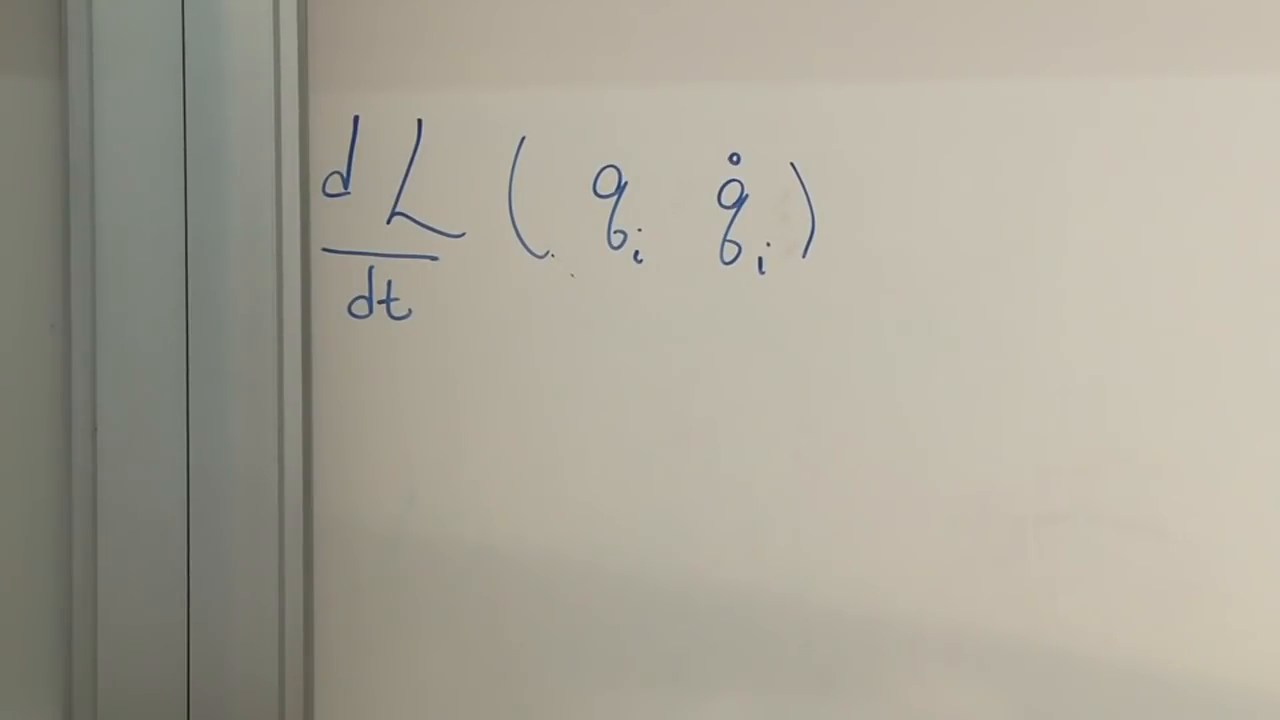
\includegraphics[width=0.72\textwidth]{lecture_05_figure_02.png}
  \caption{궤적을 따라 \(L(q_i,\dot q_i)\)를 미분하기 시작한다.}
  \lectureframe{01:08:51}
\end{figure}

\begin{classroomqa}
  \audiencequestion{연쇄법칙을 쓴 식에서 합 기호가 빠진 것 아닌가요?
  \lecturetimestamp{01:10:39--01:11:05}}
  \lecturerresponse{그렇다. 각 좌표와 각 속도가 라그랑지안을 바꿀 수 있으므로 두 항 모두 \(i\)에 대해 합해야 한다.}
\end{classroomqa}

정준 운동량과 오일러--라그랑주 방정식을 쓰면,
\begin{equation}
  p_i=\frac{\partial L}{\partial\dot q_i},
  \qquad
  \dot p_i=\frac{\partial L}{\partial q_i}.
  \label{eq:l5-p-and-pdot}
\end{equation}
식~\eqref{eq:l5-chain-rule-no-time}은 다음과 같이 된다.
\begin{align}
  \frac{dL}{dt}
  &=\sum_i(\dot p_i\dot q_i+p_i\ddot q_i)
  \notag\\
  &=\frac{d}{dt}\sum_i p_i\dot q_i.
  \label{eq:l5-product-rule}
\end{align}
여기서 ``마법''은 곱의 미분법일 뿐이다.

\begin{figure}[htbp]
  \centering
  \includegraphics[width=0.84\textwidth]{lecture_05_figure_21.png}
  \caption{운동 방정식을 이용해 연쇄법칙을 \(\sum_i p_i\dot q_i\)의 도함수로 바꾸었다.}
  \lectureframe{01:13:45}
\end{figure}

\begin{classroomqa}
  \audiencequestion{마지막 곱에서 \(q_i\)에는 점이 하나 붙나요, 둘 붙나요?
  \lecturetimestamp{01:14:31--01:15:32}}
  \lecturerresponse{곱 안에서는 점 하나가 붙은 \(p_i\dot q_i\)이다. 곱을 미분하면 \(\dot p_i\dot q_i+p_i\ddot q_i\)가 되므로, 전개된 두 번째 항에 점이 두 개 붙는 이유를 알 수 있다.}
\end{classroomqa}

두 도함수를 빼면 보존되는 조합을 얻는다. 관례에 따라 그 음수를 택해 해밀토니안이라고 부른다.
\begin{equation}
  H=\sum_i p_i\dot q_i-L.
  \label{eq:l5-hamiltonian-definition}
\end{equation}

\begin{figure}[htbp]
  \centering
  \includegraphics[width=0.80\textwidth]{lecture_05_figure_22.png}
  \caption{보존되는 조합 \(L-\sum_i p_i\dot q_i=-H\)과 해밀토니안의 정의.}
  \lectureframe{01:18:05}
\end{figure}

퍼텐셜 안의 입자 하나에 대해서는,
\begin{equation}
  L=\frac12m\dot x^2-V(x),
  \qquad p=m\dot x.
  \label{eq:l5-particle-lagrangian}
\end{equation}
따라서
\begin{align}
  H&=p\dot x-L
  \notag\\
   &=m\dot x^2-\left(\frac12m\dot x^2-V(x)\right)
  \notag\\
   &=\frac12m\dot x^2+V(x)=T+V.
  \label{eq:l5-particle-energy}
\end{align}

\begin{figure}[htbp]
  \centering
  \includegraphics[width=0.86\textwidth]{lecture_05_figure_23.png}
  \caption{퍼텐셜 안에 있는 입자의 해밀토니안은 익숙한 운동에너지와 퍼텐셜 에너지의 합으로 환원된다.}
  \lectureframe{01:20:50}
\end{figure}

이 유도 과정에서는 \(L\)의 특정한 형태를 가정하지 않았다. 따라서 이 형식론에서 에너지의 일반적인 정의는 \(T+V\)가 아니라 식~\eqref{eq:l5-hamiltonian-definition}이다.

\section{명시적 시간 의존성과 에너지 교환}

연쇄법칙에 명시적인 시간 의존성을 다시 포함하면,
\begin{equation}
  \frac{dL}{dt}
  =\sum_i\left(
    \frac{\partial L}{\partial q_i}\dot q_i
    +\frac{\partial L}{\partial\dot q_i}\ddot q_i
  \right)
  +\frac{\partial L}{\partial t}.
  \label{eq:l5-full-chain-rule}
\end{equation}
좌변은 운동을 따라 취한 전미분이다. 마지막 편미분은 \(q\)와 \(\dot q\)를 고정한 채 외부에서 변하는 매개변수만 미분한다. 같은 곱의 미분법을 적용하면 다음을 얻는다.
\begin{equation}
  \boxed{\frac{dH}{dt}=-\frac{\partial L}{\partial t}}.
  \label{eq:l5-hamiltonian-time}
\end{equation}

\begin{figure}[htbp]
  \centering
  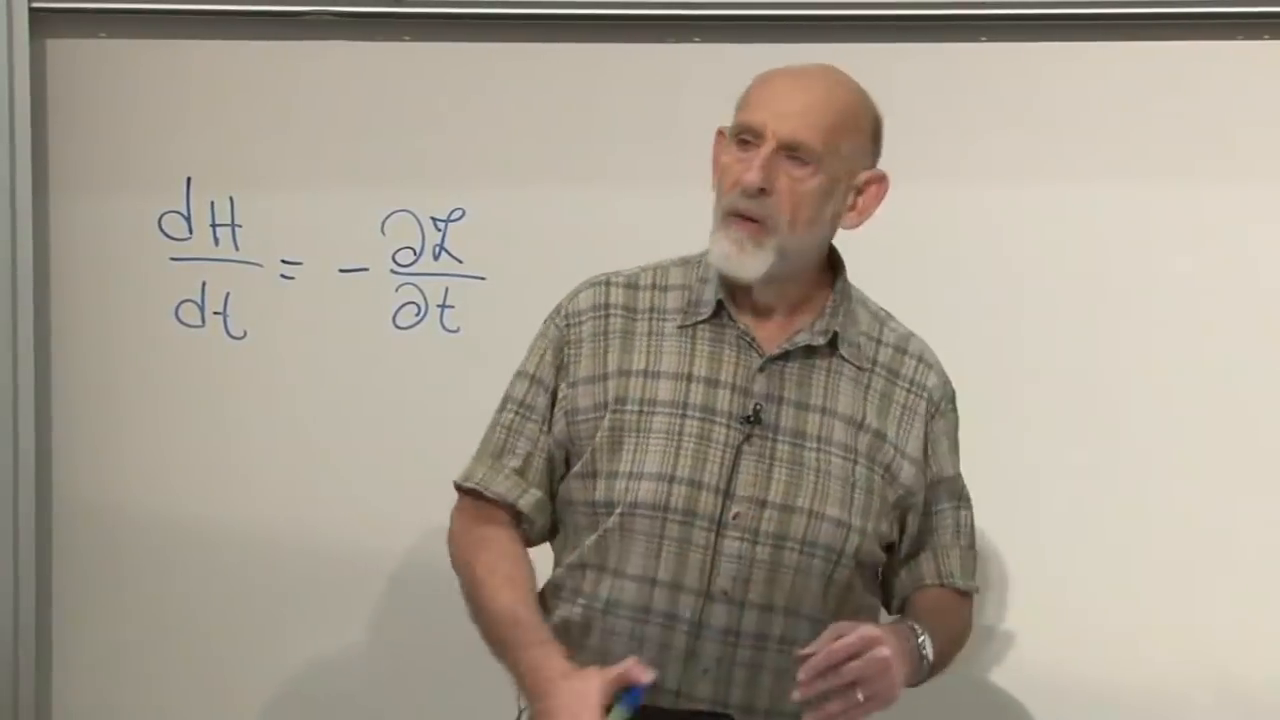
\includegraphics[width=0.70\textwidth]{lecture_05_figure_04.png}
  \caption{해밀토니안은 라그랑지안의 명시적 시간 의존성을 통해서만 변한다.}
  \lectureframe{01:37:22}
\end{figure}

식~\eqref{eq:l5-driven-oscillator}의 구동 조화 진동자에서는
\begin{equation}
  \frac{\partial L}{\partial t}
  =-\frac12\dot k(t)x^2,
  \qquad
  \dot H=\frac12\dot k(t)x^2.
  \label{eq:l5-driven-energy-rate}
\end{equation}
\(x=0\)에서는 순간 변화율이 사라진다. 원점에서 벗어나면 스프링 상수를 바꿀 때 \(x^2\dot k\)에 비례하는 비율로 일이 이루어진다.

\begin{classroomqa}
  \audiencequestion{에너지가 보존되지 않는다면 에너지는 해밀토니안의 시간 미분으로 정의되나요?
  \lecturetimestamp{01:27:11--01:28:04}}
  \lecturerresponse{아니다. 에너지는 \(H\)이다. 그 도함수는 에너지가 어떻게 변하는지를 알려 준다. 라그랑지안이 익숙한 형태이면 \(H=T+V\)이고, 그렇지 않으면 식~\eqref{eq:l5-hamiltonian-definition}이 정의를 준다. 외부 구동 장치를 포함하도록 계를 확장하면 전체 해밀토니안은 다시 보존된다.}
\end{classroomqa}

\begin{classroomqa}
  \audiencequestion{앞서 원심력과 코리올리 항이 등장한 회전 회전목마 위의 관찰자 문제에는 어떻게 적용되나요?
  \lecturetimestamp{01:28:08--01:29:52}}
  \lecturerresponse{일정하게 회전하는 좌표계는 시간에 따라 변하는 변수 변환이지, 고정된 공간 대칭도 단순한 시간 병진도 아니다. 변환된 라그랑지안으로 해밀토니안을 구성할 수 있지만, 대수 전개가 자기력 논의와 밀접하게 관련된 형태를 띠므로 그 별도 계산은 자기력을 다룰 때로 미루는 편이 낫다.}
\end{classroomqa}

\section{한눈에 보는 라그랑지안 도구}

이제 전체 구조를 간결하게 모아 쓰면 다음과 같다.
\begin{align}
  L&=L(q_i,\dot q_i,t),
  \notag\\
  p_i&=\frac{\partial L}{\partial\dot q_i},
  \qquad
  \dot p_i=\frac{\partial L}{\partial q_i},
  \notag\\
  \delta q_i&=\epsilon f_i(q)
  \quad\Longrightarrow\quad
  Q=\sum_i p_i f_i(q),\quad \dot Q=0,
  \notag\\
  H&=\sum_i p_i\dot q_i-L,
  \qquad
  \dot H=-\frac{\partial L}{\partial t}.
  \label{eq:l5-toolkit}
\end{align}

\begin{figure}[htbp]
  \centering
  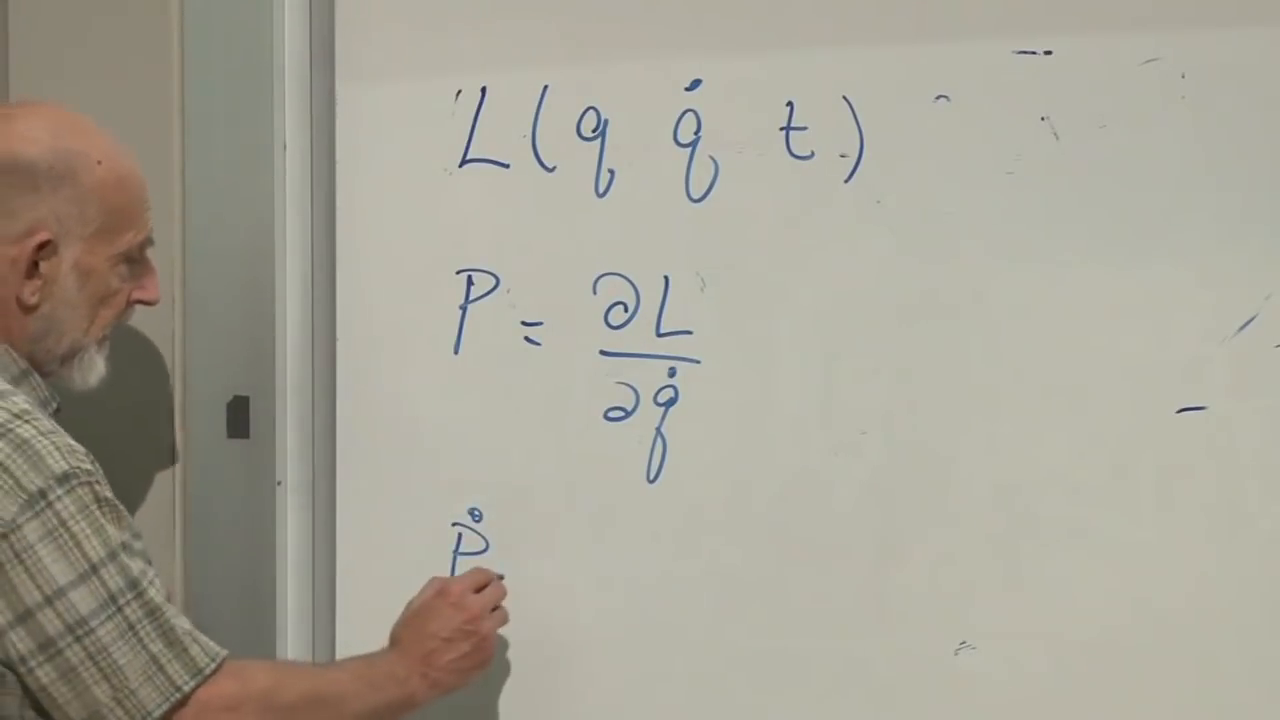
\includegraphics[width=0.66\textwidth]{lecture_05_figure_03.png}
  \caption{판서 요약은 \(L(q,\dot q,t)\), 정준 운동량, 오일러--라그랑주 방정식으로 시작한다.}
  \lectureframe{01:31:37}
\end{figure}

이 공식들에는 정의, 운동 방정식, 보통의 연속 대칭에 대응하는 전하, 시간 병진에 대응하는 전하가 담겨 있다. 특별한 요령은 많지 않다. 서로 무관한 식을 외우기보다 직접 다시 유도할 수 있는 것이 중요하다.

\section{라그랑지안 역학이나 해밀토니안 역학을 쓰는 이유}

\begin{classroomqa}
  \audiencequestion{역학은 \(L\)와 \(H\) 중 어느 쪽으로도 똑같이 기술할 수 있나요? 그렇다면 왜 한 형식을 선택하나요?
  \lecturetimestamp{01:37:16--01:39:18}}
  \lecturerresponse{르장드르 변환이 정칙이면 두 형식은 동등하지만, 강조하는 구조는 서로 다르다. 라그랑지안 형식은 정지작용 원리에서 자연스럽게 출발한다. 해밀토니안 역학은 처음에는 더 추상적이지만 방정식이 간결하고 양자역학에서 핵심적인 역할을 한다. 해밀토니안은 에너지이지만, 그 역할은 에너지 보존 법칙에만 국한되지 않는다.}
\end{classroomqa}

\begin{classroomqa}
  \audiencequestion{뉴턴은 해밀토니안 형식의 에너지 보존을 알고 있었나요?
  \lecturetimestamp{01:39:29--01:39:56}}
  \lecturerresponse{역사 기록이 보여 주는 한, 뉴턴은 이 형식으로 정식화하지 않았다. 뉴턴이 제시한 틀은 힘의 법칙 \(F=ma\)이었다.}
\end{classroomqa}

\begin{classroomqa}
  \audiencequestion{모든 물리계에 라그랑지안이 있어야 하는 이유는 무엇인가요? 그건 단지 실험적 사실인가요?
  \lecturetimestamp{01:39:57--01:42:37}}
  \lecturerresponse{여기서 다루는 폐쇄계의 경우 이는 경험적 사실이며, 더 근본적인 양자 기술에서도 따라 나온다. 수학적으로 일관되면서도 오일러--라그랑주 방정식이 아닌 미분방정식도 만들 수 있다. 예를 들어 \(\dot x=-x\)은 완전히 풀 수 있지만, 근본적인 폐쇄계의 1차원 법칙으로 보면 소산 현상처럼 정보를 잃는 성격을 가진다. 고전역학이 논리적으로 양자역학보다 앞서는 것은 아니다. 고전역학의 근본 구조는 양자역학에서 물려받는다. 자세한 이유는 뒤에서 다루겠다.}
\end{classroomqa}

\begin{classroomqa}
  \audiencequestion{실제 폐쇄계마다 라그랑지안이 있다면, 라그랑지안이라고 부르는 모든 함수가 자연에서 발견되는 계에 대응하나요?
  \lecturetimestamp{01:42:39--01:42:54}}
  \lecturerresponse{아니다. 형식적인 계산 체계에서는 알려진 어떤 물리계에서도 실현되지 않는 함수도 많이 허용한다.}
\end{classroomqa}

\begin{classroomqa}
  \audiencequestion{라그랑지안은 주로 퍼텐셜을 만들어 내는 도구인가요?
  \lecturetimestamp{01:42:54--01:43:32}}
  \lecturerresponse{그보다 쓰임이 넓다. 후보 역학계를 체계화할 수 있고, 운동 방정식을 얻는 가장 간결하고 실용적인 경로인 경우도 많다.}
\end{classroomqa}

이중진자는 그런 실용적 이점을 보여 준다. 두 각을 택하고, 그 각과 시간 미분으로 두 질량의 속도를 구해 \(T-V\)를 구성한 다음 오일러--라그랑주 방정식이 구속력을 암묵적으로 처리하게 한다. 모든 장력과 가속도를 \(F=ma\)로 하나하나 구하는 것보다 훨씬 간결하다.

\begin{figure}[htbp]
  \centering
  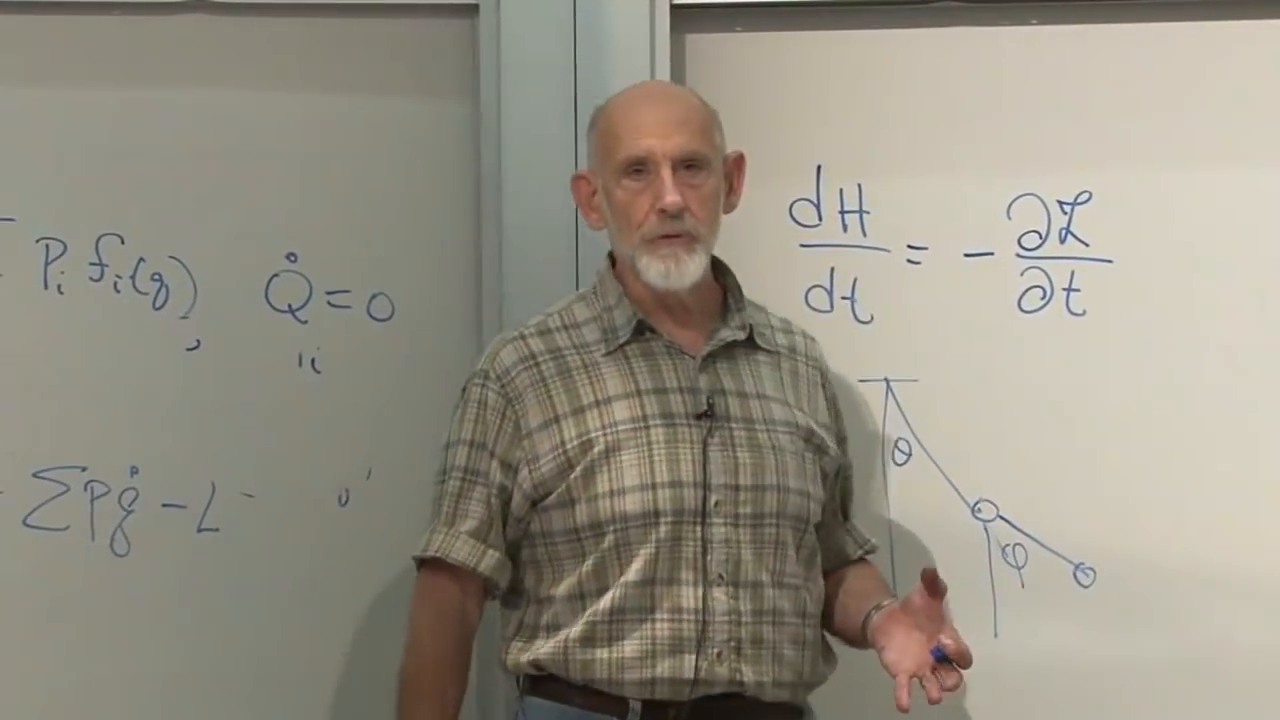
\includegraphics[width=0.84\textwidth]{lecture_05_figure_05.png}
  \caption{이중진자 그림 옆에는 에너지 변화율 항등식이 계속 남아 있다.}
  \lectureframe{01:45:39}
\end{figure}

\begin{figure}[htbp]
  \centering
  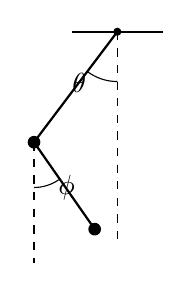
\begin{tikzpicture}[scale=1.15]
    \draw[thick] (-0.5,0) -- (0.5,0);
    \fill (0,0) circle (0.045);
    \draw[dashed] (0,0) -- (0,-2.3);
    \draw[thick] (0,0) -- (-0.92,-1.22);
    \fill (-0.92,-1.22) circle (0.07);
    \draw[dashed] (-0.92,-1.22) -- (-0.92,-2.55);
    \draw[thick] (-0.92,-1.22) -- (-0.25,-2.18);
    \fill (-0.25,-2.18) circle (0.07);
    \draw (0,-0.55) arc (-90:-127:0.55);
    \node at (-0.42,-0.56) {$\theta$};
    \draw (-0.92,-1.72) arc (-90:-55:0.48);
    \node at (-0.56,-1.72) {$\phi$};
  \end{tikzpicture}
  \caption{이중진자의 일반화된 각좌표.}
\end{figure}

변수 변환도 마찬가지로 효율적이다. 각각의 힘 방정식을 따로 변환하는 대신 라그랑지안 하나를 변환한 뒤 그에 대한 방정식을 유도하면 된다.

\begin{classroomqa}
  \audiencequestion{이중 진자는 태양, 지구, 달처럼 세 물체로 이루어진 또 다른 계에서 한 물체를 기준점으로 취급한 경우와 본질적으로 같은가요?
  \lecturetimestamp{01:45:06--01:45:25}}
  \lecturerresponse{그 비유는 계층 구조를 잘 포착하지만, 막대가 만드는 구속 조건은 다릅니다. 어느 경우든 질량이 매우 크거나 고정된 성분은 근사적으로 기준 구조로 취급할 수 있습니다.}
\end{classroomqa}

\begin{classroomqa}
  \audiencequestion{이중 진자에서는 \(T-V\)를 사용하지만, 방금 더 일반적인 라그랑지안도 강조하셨습니다. \(T-V\)는 언제 성립하나요?
  \lecturetimestamp{01:46:08--01:46:58}}
  \lecturerresponse{관성계에서 보는 보통의 비상대론적 입자에 자기장에 의한 속도 결합이 없을 때는 익숙한 형태가 적용됩니다. 회전 좌표계, 상대론적 계, 자기장이 있는 경우에는 더 일반적인 항이 필요합니다.}
\end{classroomqa}

\begin{classroomqa}
  \audiencequestion{충돌은 이 설명의 범위를 벗어나나요?
  \lecturetimestamp{01:47:00--01:48:05}}
  \lecturerresponse{탄성 충돌은 짧은 거리에서 작용하는 힘, 따라서 퍼텐셜에서 비롯됩니다. 비탄성 충돌도 미시적 수준에서는 역학적 현상이지만, 에너지는 내부 진동, 변형, 열로 들어갑니다. 이러한 자유도를 제외한 질량중심 기술은 불완전합니다.}
\end{classroomqa}

\begin{classroomqa}
  \audiencequestion{방망이에 맞은 야구공을 \(F=ma\)로 분석할 수 있나요?
  \lecturetimestamp{01:48:05--01:48:33}}
  \lecturerresponse{거친 수준에서만 가능합니다. 완전한 설명을 위해서는 변형, 가열, 공의 손상 가능성, 어쩌면 방망이가 부러지는 경우까지 다루어야 합니다. 현실적인 충돌이 점입자 충돌보다 훨씬 더 어려운 이유는 이런 내부 자유도에 있습니다.}
\end{classroomqa}

\begin{classroomqa}
  \audiencequestion{크기가 있는 강체는 어떤가요?
  \lecturetimestamp{01:48:34--01:49:00}}
  \lecturerresponse{강체는 뉴턴 역학의 방법으로 연구할 수도 있고, 병진 좌표와 회전 좌표로 쓴 \(T-V\) 라그랑지안으로 연구할 수도 있습니다. 그 라그랑지안을 구성하는 것은 유익한 연습입니다.}
\end{classroomqa}

\begin{classroomqa}
  \audiencequestion{양자역학의 에너지--시간 불확정성 관계는 에너지가 엄밀히 보존되지 않는다는 뜻인가요?
  \lecturetimestamp{01:49:01--01:49:29}}
  \lecturerresponse{아닙니다. 에너지는 엄밀히 보존될 수 있습니다. 이 관계가 말하는 것은 에너지를 높은 정확도로 알아내려면 오랜 시간 관측해야 한다는 점입니다. 이 관계가 보존 법칙을 대체하는 것은 아닙니다.}
\end{classroomqa}

\begin{classroomqa}
  \audiencequestion{뉴턴 역학과 라그랑주 역학은 논리적으로 동등한가요?
  \lecturetimestamp{01:49:36--01:50:07}}
  \lecturerresponse{두 정식화가 모두 적용되는 통상적인 영역에서는 동등합니다. 그렇더라도 기본적인 형태 \(m\ddot x=F(x)\)와 닮지 않은 운동 방정식을 주는 라그랑지안을 만들어낼 수는 있습니다.}
\end{classroomqa}

\section{좌표에 의존하는 운동에너지 항}

일부러 낯설게 만든 다음 예를 살펴봅시다.
\begin{equation}
  L=\frac12q^2\dot q^2-\frac12q^2.
  \label{eq:l5-nonstandard-l}
\end{equation}
이는 좌표에 의존하는 운동에너지 계수를 가진 유효한 라그랑지안입니다. \(q\dot q\)와 같이 속도에 선형인 항도 생각할 수 있습니다. 이 1차원 예에서 그 항은 전미분이므로 운동 방정식을 바꾸지 않습니다.

정준 운동량은 다음과 같습니다.
\begin{equation}
  p=\frac{\partial L}{\partial\dot q}=q^2\dot q,
  \label{eq:l5-nonstandard-p}
\end{equation}
따라서
\begin{equation}
  \dot p=q^2\ddot q+2q\dot q^2,
  \qquad
  \frac{\partial L}{\partial q}=q\dot q^2-q.
  \label{eq:l5-nonstandard-derivatives}
\end{equation}
운동 방정식은 다음과 같습니다.
\begin{equation}
  q^2\ddot q+q\dot q^2=-q.
  \label{eq:l5-nonstandard-eom}
\end{equation}

\begin{figure}[htbp]
  \centering
  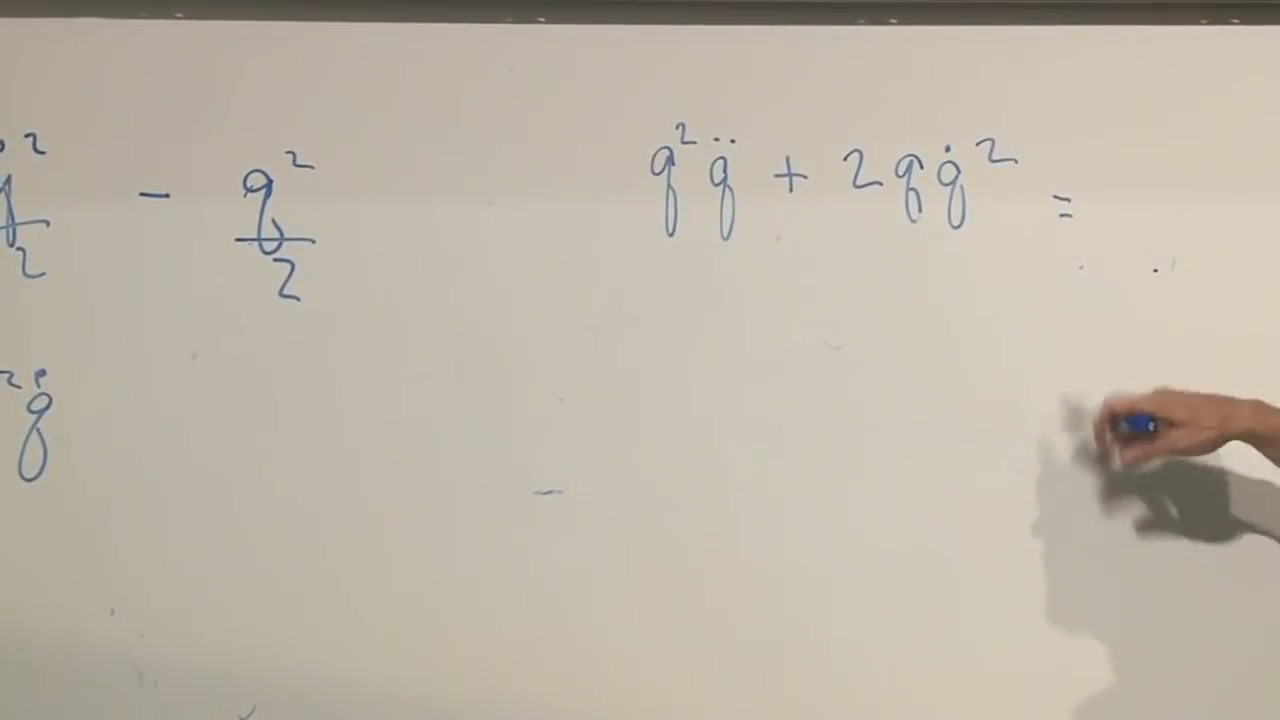
\includegraphics[width=0.80\textwidth]{lecture_05_figure_06.png}
  \caption{좌표 의존적 운동에너지 예에서 미분한 운동량.}
  \lectureframe{01:52:32}
\end{figure}

\begin{classroomqa}
  \audiencequestion{이 방정식을 \(q\)로 나누어도 되나요?
  \lecturetimestamp{01:53:22--01:53:39}}
  \lecturerresponse{\(q\neq0\)인 경우에만 가능합니다. \(q=0\)에서는 운동에너지 계수와 르장드르 사상이 퇴화하므로, 나누면 별도로 다뤄야 하는 특이점을 누락하게 됩니다.}
\end{classroomqa}

해밀토니안은 다음과 같습니다.
\begin{align}
  H&=p\dot q-L
  \notag\\
   &=q^2\dot q^2-
     \left(\frac12q^2\dot q^2-\frac12q^2\right)
  \notag\\
   &=\frac12q^2\dot q^2+\frac12q^2.
  \label{eq:l5-nonstandard-h}
\end{align}

\begin{classroomqa}
  \audiencequestion{그래도 \(q^2\dot q^2/2\)를 운동에너지라고 부를 수 있나요?
  \lecturetimestamp{01:54:41--01:55:07}}
  \lecturerresponse{네. 이 계산 예에서 해밀토니안은 다시 양의 운동에너지 항과 퍼텐셜 항의 합처럼 보입니다. 여기서 중요한 점은 기본적인 상수 질량 형태를 먼저 가정하지 않아도 형식적 정의가 작동했다는 것입니다.}
\end{classroomqa}

\section{소산과 형식의 더 깊은 기원}

\begin{classroomqa}
  \audiencequestion{마찰은 라그랑지안에 어떻게 포함하나요?
  \lecturetimestamp{01:55:09--01:56:17}}
  \lecturerresponse{여기서 다루는 단순한 폐쇄계, 즉 자유도가 유한한 계에서는 마찰을 근본적인 힘으로 포함하지 않습니다. 거시적 마찰은 엄청나게 많은 미시적 자유도의 통계적 효과입니다. 그 원자가 여전히 기저 역학을 따르지만, 원자를 추적하지 않는 축약된 기술에서는 소산이 나타납니다.}
\end{classroomqa}

\begin{classroomqa}
  \audiencequestion{해밀턴은 어떻게 자신의 정식화에 이르렀나요?
  \lecturetimestamp{01:56:22--01:56:37}}
  \lecturerresponse{여기서는 역사적 유도를 제시하지 않았습니다. 이 강의에서 중요한 과제는 그 정식화가 어떻게 작동하는지 이해하는 것입니다.}
\end{classroomqa}

\begin{classroomqa}
  \audiencequestion{라그랑지안이 눈에 띄게 \(T-V\) 형태가 아닐 때, 이를 구하는 더 일반적인 방법이 있나요?
  \lecturetimestamp{01:56:43--01:58:54}}
  \lecturerresponse{실험, 근거 있는 추측, 대칭 원리, 또는 원하는 방정식으로부터의 재구성을 통해 함수를 정할 수 있습니다. 미적분학 자체에 그 입력이 어디서 오는지 묻는 것은 도함수의 정의에 \(f(x)\)가 어디서 왔는지 묻는 것과 같습니다. 함수가 주어진 뒤에 무엇을 해야 하는지는 미적분학이 알려줍니다. 자연의 폐쇄계가 왜 이 추상적 구조를 따르는지는 양자역학이 더 깊은 수준에서 답합니다.}
\end{classroomqa}

이 점은 강의의 도입부에서 다룬 주제와 연결됩니다. 근본적인 해밀토니안 시간 변화는 궤적이 서로 합쳐지지 않고 정보가 단순히 소멸하지 않는다는 의미에서 결정론적이고 가역적입니다. 이 성질과 위상 공간 정식화의 관계는 단계적으로 전개할 것입니다.

\begin{classroomqa}
  \audiencequestion{변분법은 원하는 고전 방정식에서 역으로 거슬러 올라가 작동했을 뿐인가요? 양자역학도 같은 방식으로 라그랑지안을 얻나요?
  \lecturetimestamp{01:59:37--02:01:07}}
  \lecturerresponse{기초적인 고전역학의 구성에서는 알려진 방정식을 정지 경로로 재현하는 작용을 실제로 선택할 수 있습니다. 양자역학에서는 논리적 순서가 다릅니다. 양자역학은 자연스럽게 해밀토니안에서 출발해 라그랑지안 기술로 나아갈 수 있습니다. 고전역학에서 해밀토니안은 처음에는 추상적으로 보이지만, 양자역학에서는 더 직관적입니다.}
\end{classroomqa}

\begin{classroomqa}
  \audiencequestion{양자역학으로 마찰을 기술할 수 있나요?
  \lecturetimestamp{02:01:08--02:02:05}}
  \lecturerresponse{네. 다만 근본적인 기술에는 환경의 자유도를 포함해야 합니다. 점성이 있는 유체 속에서 움직이는 입자를 완전히 기술하려면 유체를 이루는 입자들도 고려해야 합니다. 마찰은 그 자유도를 하나씩 추적하지 않을 때 나타나는 복잡한 집단 효과입니다.}
\end{classroomqa}
